\documentclass{beamer}

\setlength{\parskip}{\baselineskip}
\setlength{\parindent}{0pt}
\usepackage{default}
\usepackage{tabularx}
\usepackage{url}
\usepackage{graphicx}

\title{\huge{Using \texttt{bitbucket} for collaboration with international colleagues}}
\author{Manuel Baumann}
\titlegraphic{
   \vspace{-0.8cm}
\includegraphics[scale=0.08]{images/TU_Delft_logo1.png}\hspace{4cm}\includegraphics[scale=0.15]{../../images/logo}}
\date{\footnotesize{October 30, 2014}}
\begin{document}

\frame{
\titlepage
}

\begin{frame}
\frametitle{First, some announcements}
\vspace{1cm}
\textit{This is the first ba\color{red}NaN\color{black}a talk in the framework of our new SIAM student chapter.}
\begin{itemize}
 \item Visit Tata Steel on Nov. 21, 2014
 \pause
 \item Student Krylov Day on Febr. 2, 2015
 \pause
 \item Next ba\color{red}NaN\color{black}a talks: Reinaldo (LAPACK) and Xiaozhou (Python)
\end{itemize}
\begin{figure}
\hfill 
\includegraphics[scale=0.12]{images/SSC_Delft_new}
\end{figure}

\end{frame}

\begin{frame}
\frametitle{Today's lecture: \texttt{git} + \texttt{bitbucket}}
Do you know this situation?
\begin{figure}
\centering
 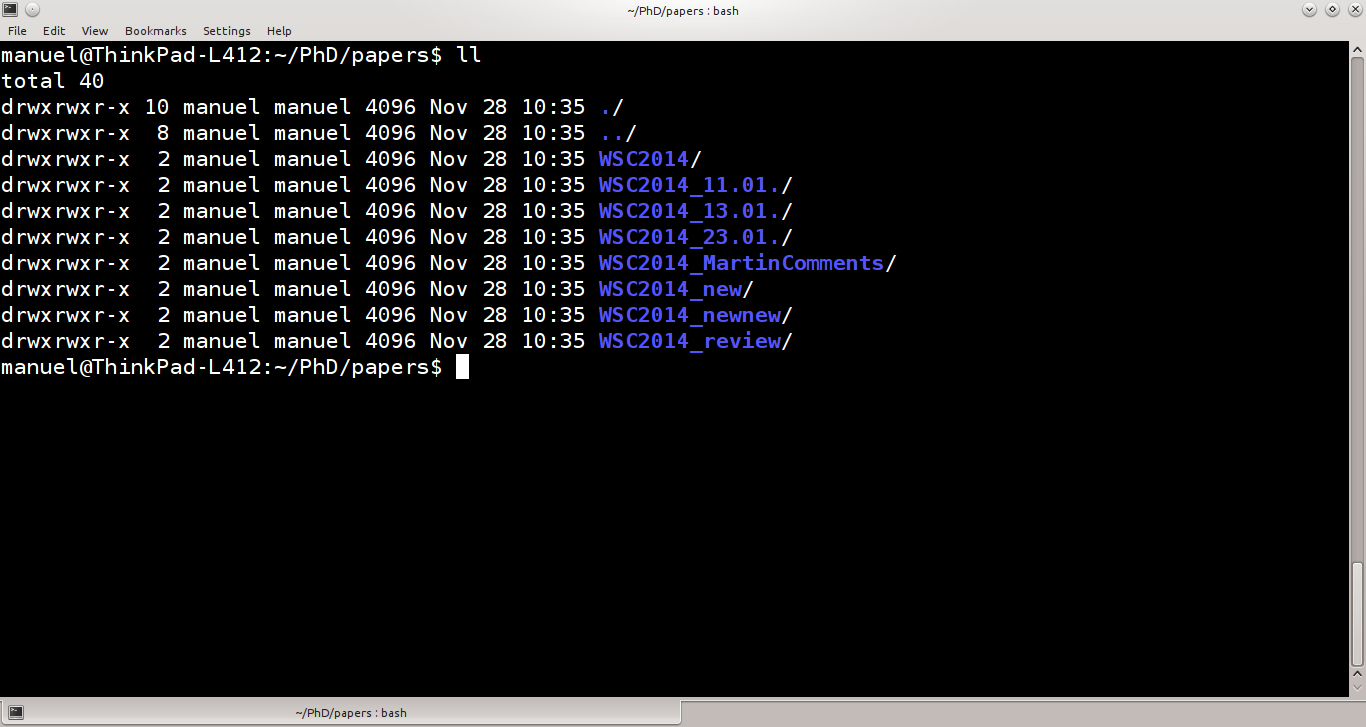
\includegraphics[height=0.6\textheight]{images/screnshot1.png}
\end{figure}
\end{frame}

\begin{frame}
\frametitle{Recap: \texttt{git}}
The pre-installed software package \texttt{git} can be used for version control for a (bigger) software project.
\begin{itemize}
 \item helps to keep track of changes in your project directory
 \item branching, merging
 \item collaboration
 \item several sites allow you to publish your \texttt{git} repository (github, bitbucket, gitorious) 
\end{itemize}
\end{frame}

\begin{frame}
\frametitle{Git basics}
Git stores snapshots (called \emph{commits} in git) of files in a repository.

A commit consists of
\begin{itemize}
 \item a set of files,
 \item a message,
 \item an author,
 \item a date,
 \item references to one or more parent commits and
 \item a hash (of the above).
\end{itemize}

You are in control of creating commits!
\end{frame}

\begin{frame}[fragile]
\frametitle{Git basics}
\begin{description}[working directory]
 \item[working directory]
  Plain directory where you can edit files using your favourite editor.
 \item[staging area]
  Area listing the files to be commited.
 \item[repository]
  Collection of commits.
\end{description}

Everything is stored locally (in the working directory):
\begin{description}[working directory]
 \item[repository] \verb|working_directory/.git|
 \item[staging area] \verb|working_directory/.git/index|
\end{description}
\end{frame}

\begin{frame}
\frametitle{Basic commands}
\begin{table}
\begin{tabularx}{\textwidth}{l|X}
Command & Meaning \\
 \hline
 \texttt{git init} & First command, makes current folder a \texttt{git} repository\\
 \texttt{git add <file>} & Stages a file\\
 \texttt{git commit -m <message>} & Record changes to the repository\\
 \texttt{git status} & Show the working tree status\\
 \texttt{git diff} & Show changes between commits, commit and working tree, etc\\
 \texttt{git log} & Show commit logs\\
\end{tabularx}
\end{table}
\hfill $\hookrightarrow$ live demonstration...
\end{frame}

\begin{frame}
\frametitle{Branches}
\begin{itemize}
 \item Branching is the git-equivalent of making a copy of your working
 directory.
 \item Branching is cheap.  Use it whenever you can.
 \item Git is very good in merging (two or more) branches.
 \item NOTE: Your working directory points to only one branch.
\end{itemize}
\end{frame}

\begin{frame}
\frametitle{Commands for branching and merging}
\begin{table}
\begin{tabularx}{\textwidth}{l|X}
Command & Meaning \\
 \hline
 \texttt{git branch} & List, create, or delete branches\\
 \texttt{git checkout} & Checkout a branch or paths to the working tree\\
 \texttt{git merge} & Join two or more development histories together\\
 \texttt{git mergetool} & Run merge conflict resolution tools to resolve merge conflicts\\
\end{tabularx}
\end{table}
\hfill $\hookrightarrow$ live demonstration...
\end{frame}

\begin{frame}
 \frametitle{Some notes on \texttt{bitbucket}}
 \vspace{1.5cm}
 \texttt{bitbucket.org} is a place to store your repository.
 \begin{itemize}
  \item repos is \textit{private}
  \item browser-based
  \item Some nice features: Wiki, issues, ...
  \item almost unlimited space
 \end{itemize}
\begin{figure}
\hfill 
\includegraphics[scale=0.35]{images/bitbucket-logo}
\end{figure}
\end{frame}


% \begin{frame}
% \frametitle{Today's message}
% 
% The overall message is:
% \begin{center}
%  \textit{Using git is optimal for collaborations and big software projects.}
% \end{center}
% Moreover,
% \begin{itemize}
%  \item sensitive information should not be stored in e.g. Dropbox
%  \item \texttt{git} branches are non-linear in time
%  \item local argument: \texttt{git} is supported (and pre-installed) at TU Delft work stations
% \end{itemize}
% \end{frame}
\begin{frame}
\frametitle{Further reading}
Many information are available online:
\begin{itemize}
 \item \url{https://bitbucket.org/}
 \item \url{http://try.github.io/levels/1/challenges/1}
 \item \url{http://git-scm.com/book}
\end{itemize}
These slides, and much more, will be published at:
\begin{itemize}
 \item \url{http://projectbanana.github.io/}
\end{itemize}
 \begin{figure}
\centering
 \includegraphics[height=0.3\textheight]{../../images/logo}
\end{figure}
\end{frame}

\end{document}
